%
% This is an example LaTeX file which uses the SANDreport class file.
% It shows how a SAND report should be formatted, what sections and
% elements it should contain, and how to use the SANDreport class.
% It uses the LaTeX article class, but not the strict option.
% ItINLreport uses .eps logos and files to show how pdflatex can be used
%
% Get the latest version of the class file and more at
%    http://www.cs.sandia.gov/~rolf/SANDreport
%
% This file and the SANDreport.cls file are based on information
% contained in "Guide to Preparing {SAND} Reports", Sand98-0730, edited
% by Tamara K. Locke, and the newer "Guide to Preparing SAND Reports and
% Other Communication Products", SAND2002-2068P.
% Please send corrections and suggestions for improvements to
% Rolf Riesen, Org. 9223, MS 1110, rolf@cs.sandia.gov
%
\documentclass[pdf,12pt]{../../user_manual/INLreport}
% pslatex is really old (1994).  It attempts to merge the times and mathptm packages.
% My opinion is that it produces a really bad looking math font.  So why are we using it?
% If you just want to change the text font, you should just \usepackage{times}.
% \usepackage{pslatex}
\usepackage{times}
\usepackage{longtable}
\usepackage[FIGBOTCAP,normal,bf,tight]{subfigure}
\usepackage{amsmath}
\usepackage{amssymb}
\usepackage[labelfont=bf]{caption}
\usepackage{pifont}
\usepackage{enumerate}
\usepackage{listings}
\usepackage{fullpage}
\usepackage{xcolor}          % Using xcolor for more robust color specification
\usepackage{ifthen}          % For simple checking in newcommand blocks
\usepackage{textcomp}
%\usepackage{authblk}         % For making the author list look prettier
%\renewcommand\Authsep{,~\,}

% Custom colors
\definecolor{deepblue}{rgb}{0,0,0.5}
\definecolor{deepred}{rgb}{0.6,0,0}
\definecolor{deepgreen}{rgb}{0,0.5,0}
\definecolor{forestgreen}{RGB}{34,139,34}
\definecolor{orangered}{RGB}{239,134,64}
\definecolor{darkblue}{rgb}{0.0,0.0,0.6}
\definecolor{gray}{rgb}{0.4,0.4,0.4}

\lstset {
  basicstyle=\ttfamily,
  frame=single
}

\setcounter{secnumdepth}{5}
\lstdefinestyle{XML} {
    language=XML,
    extendedchars=true,
    breaklines=true,
    breakatwhitespace=true,
%    emph={name,dim,interactive,overwrite},
    emphstyle=\color{red},
    basicstyle=\ttfamily,
%    columns=fullflexible,
    commentstyle=\color{gray}\upshape,
    morestring=[b]",
    morecomment=[s]{<?}{?>},
    morecomment=[s][\color{forestgreen}]{<!--}{-->},
    keywordstyle=\color{cyan},
    stringstyle=\ttfamily\color{black},
    tagstyle=\color{darkblue}\bf\ttfamily,
    morekeywords={name,type},
%    morekeywords={name,attribute,source,variables,version,type,release,x,z,y,xlabel,ylabel,how,text,param1,param2,color,label},
}
\lstset{language=python,upquote=true}

\usepackage{titlesec}
\newcommand{\sectionbreak}{\clearpage}
\setcounter{secnumdepth}{4}

%\titleformat{\paragraph}
%{\normalfont\normalsize\bfseries}{\theparagraph}{1em}{}
%\titlespacing*{\paragraph}
%{0pt}{3.25ex plus 1ex minus .2ex}{1.5ex plus .2ex}

%%%%%%%% Begin comands definition to input python code into document
\usepackage[utf8]{inputenc}

% Default fixed font does not support bold face
\DeclareFixedFont{\ttb}{T1}{txtt}{bx}{n}{9} % for bold
\DeclareFixedFont{\ttm}{T1}{txtt}{m}{n}{9}  % for normal

\usepackage{listings}

% Python style for highlighting
\newcommand\pythonstyle{\lstset{
language=Python,
basicstyle=\ttm,
otherkeywords={self, none, return},             % Add keywords here
keywordstyle=\ttb\color{deepblue},
emph={MyClass,__init__},          % Custom highlighting
emphstyle=\ttb\color{deepred},    % Custom highlighting style
stringstyle=\color{deepgreen},
frame=tb,                         % Any extra options here
showstringspaces=false            %
}}


% Python environment
\lstnewenvironment{python}[1][]
{
\pythonstyle
\lstset{#1}
}
{}

% Python for external files
\newcommand\pythonexternal[2][]{{
\pythonstyle
\lstinputlisting[#1]{#2}}}

\lstnewenvironment{xml}
{}
{}

% Python for inline
\newcommand\pythoninline[1]{{\pythonstyle\lstinline!#1!}}

% Named Colors for the comments below (Attempted to match git symbol colors)
\definecolor{RScolor}{HTML}{8EB361}  % Sonat (adjusted for clarity)
\definecolor{DPMcolor}{HTML}{E28B8D} % Dan
\definecolor{JCcolor}{HTML}{82A8D9}  % Josh (adjusted for clarity)
\definecolor{AAcolor}{HTML}{8D7F44}  % Andrea
\definecolor{CRcolor}{HTML}{AC39CE}  % Cristian
\definecolor{RKcolor}{HTML}{3ECC8D}  % Bob (adjusted for clarity)
\definecolor{DMcolor}{HTML}{276605}  % Diego (adjusted for clarity)
\definecolor{PTcolor}{HTML}{990000}  % Paul

\def\DRAFT{} % Uncomment this if you want to see the notes people have been adding
% Comment command for developers (Should only be used under active development)
\ifdefined\DRAFT
  \newcommand{\nameLabeler}[3]{\textcolor{#2}{[[#1: #3]]}}
\else
  \newcommand{\nameLabeler}[3]{}
\fi
\newcommand{\alfoa}[1] {\nameLabeler{Andrea}{AAcolor}{#1}}
\newcommand{\cristr}[1] {\nameLabeler{Cristian}{CRcolor}{#1}}
\newcommand{\mandd}[1] {\nameLabeler{Diego}{DMcolor}{#1}}
\newcommand{\maljdan}[1] {\nameLabeler{Dan}{DPMcolor}{#1}}
\newcommand{\cogljj}[1] {\nameLabeler{Josh}{JCcolor}{#1}}
\newcommand{\bobk}[1] {\nameLabeler{Bob}{RKcolor}{#1}}
\newcommand{\senrs}[1] {\nameLabeler{Sonat}{RScolor}{#1}}
\newcommand{\talbpaul}[1] {\nameLabeler{Paul}{PTcolor}{#1}}
% Commands for making the LaTeX a bit more uniform and cleaner
\newcommand{\TODO}[1]    {\textcolor{red}{\textit{(#1)}}}
\newcommand{\xmlAttrRequired}[1] {\textcolor{red}{\textbf{\texttt{#1}}}}
\newcommand{\xmlAttr}[1] {\textcolor{cyan}{\textbf{\texttt{#1}}}}
\newcommand{\xmlNodeRequired}[1] {\textcolor{deepblue}{\textbf{\texttt{<#1>}}}}
\newcommand{\xmlNode}[1] {\textcolor{darkblue}{\textbf{\texttt{<#1>}}}}
\newcommand{\xmlString}[1] {\textcolor{black}{\textbf{\texttt{'#1'}}}}
\newcommand{\xmlDesc}[1] {\textbf{\textit{#1}}} % Maybe a misnomer, but I am
                                                % using this to detail the data
                                                % type and necessity of an XML
                                                % node or attribute,
                                                % xmlDesc = XML description
\newcommand{\default}[1]{~\\*\textit{Default: #1}}
\newcommand{\nb} {\textcolor{deepgreen}{\textbf{~Note:}}~}

%%%%%%%% End comands definition to input python code into document

%\usepackage[dvips,light,first,bottomafter]{draftcopy}
%\draftcopyName{Sample, contains no OUO}{70}
%\draftcopyName{Draft}{300}

% The bm package provides \bm for bold math fonts.  Apparently
% \boldsymbol, which I used to always use, is now considered
% obsolete.  Also, \boldsymbol doesn't even seem to work with
% the fonts used in this particular document...
\usepackage{bm}

% Define tensors to be in bold math font.
\newcommand{\tensor}[1]{{\bm{#1}}}

% Override the formatting used by \vec.  Instead of a little arrow
% over the letter, this creates a bold character.
\renewcommand{\vec}{\bm}

% Define unit vector notation.  If you don't override the
% behavior of \vec, you probably want to use the second one.
\newcommand{\unit}[1]{\hat{\bm{#1}}}
% \newcommand{\unit}[1]{\hat{#1}}

% Use this to refer to a single component of a unit vector.
\newcommand{\scalarunit}[1]{\hat{#1}}

% \toprule, \midrule, \bottomrule for tables
\usepackage{booktabs}

% \llbracket, \rrbracket
\usepackage{stmaryrd}

\usepackage{hyperref}
\hypersetup{
    colorlinks,
    citecolor=black,
    filecolor=black,
    linkcolor=black,
    urlcolor=black
}

\newcommand{\wiki}{\href{https://github.com/idaholab/hybrid/wiki}{HYBRID wiki}}

% Compress lists of citations like [33,34,35,36,37] to [33-37]
\usepackage{cite}

% If you want to relax some of the SAND98-0730 requirements, use the "relax"
% option. It adds spaces and boldface in the table of contents, and does not
% force the page layout sizes.
% e.g. \documentclass[relax,12pt]{SANDreport}
%
% You can also use the "strict" option, which applies even more of the
% SAND98-0730 guidelines. It gets rid of section numbers which are often
% useful; e.g. \documentclass[strict]{SANDreport}

% The INLreport class uses \flushbottom formatting by default (since
% it's intended to be two-sided document).  \flushbottom causes
% additional space to be inserted both before and after paragraphs so
% that no matter how much text is actually available, it fills up the
% page from top to bottom.  My feeling is that \raggedbottom looks much
% better, primarily because most people will view the report
% electronically and not in a two-sided printed format where some argue
% \raggedbottom looks worse.  If we really want to have the original
% behavior, we can comment out this line...
\raggedbottom
\setcounter{secnumdepth}{5} % show 5 levels of subsection
\setcounter{tocdepth}{5} % include 5 levels of subsection in table of contents

% ---------------------------------------------------------------------------- %
%
% Set the title, author, and date
%
\title{HYBRID Software Design Description}

\author{Konor Frick, Andrea Alfonsi}
 

% There is a "Printed" date on the title page of a SAND report, so
% the generic \date should [WorkingDir:]generally be empty.
\date{}


% ---------------------------------------------------------------------------- %
% Set some things we need for SAND reports. These are mandatory
%
\SANDnum{SDD-561}
\SANDprintDate{\today}
\SANDauthor{Konor Frick, Andrea Alfonsi}
\SANDreleaseType{Revision 0}

% ---------------------------------------------------------------------------- %
% Include the markings required for your SAND report. The default is "Unlimited
% Release". You may have to edit the file included here, or create your own
% (see the examples provided).
%
% \include{MarkOUO} % Not needed for unlimted release reports

\def\component#1{\texttt{#1}}

% ---------------------------------------------------------------------------- %
\newcommand{\systemtau}{\tensor{\tau}_{\!\text{SUPG}}}

% Added by Sonat
\usepackage{placeins}
\usepackage{array}

\newcolumntype{L}[1]{>{\raggedright\let\newline\\\arraybackslash\hspace{0pt}}m{#1}}
\newcolumntype{C}[1]{>{\centering\let\newline\\\arraybackslash\hspace{0pt}}m{#1}}
\newcolumntype{R}[1]{>{\raggedleft\let\newline\\\arraybackslash\hspace{0pt}}m{#1}}

% end added by Sonat
% ---------------------------------------------------------------------------- %
%
% Start the document
%

\begin{document}
    \maketitle

    % ------------------------------------------------------------------------ %
    % An Abstract is required for SAND reports
    %
%    \begin{abstract}
%    \input abstract
%    \end{abstract}


    % ------------------------------------------------------------------------ %
    % An Acknowledgement section is optional but important, if someone made
    % contributions or helped beyond the normal part of a work assignment.
    % Use \section* since we don't want it in the table of context
    %
%    \clearpage
%    \section*{Acknowledgment}



%	The format of this report is based on information found
%	in~\cite{Sand98-0730}.


    % ------------------------------------------------------------------------ %
    % The table of contents and list of figures and tables
    % Comment out \listoffigures and \listoftables if there are no
    % figures or tables. Make sure this starts on an odd numbered page
    %
    \cleardoublepage		% TOC needs to start on an odd page
    \tableofcontents
    %\listoffigures
    %\listoftables


    % ---------------------------------------------------------------------- %
    % An optional preface or Foreword
%    \clearpage
%    \section*{Preface}
%    \addcontentsline{toc}{section}{Preface}
%	Although muggles usually have only limited experience with
%	magic, and many even dispute its existence, it is worthwhile
%	to be open minded and explore the possibilities.


    % ---------------------------------------------------------------------- %
    % An optional executive summary
    %\clearpage
    %\section*{Summary}
    %\addcontentsline{toc}{section}{Summary}
    %\input{Summary.tex}
%	Once a certain level of mistrust and skepticism has
%	been overcome, magic finds many uses in todays science



%	and engineering. In this report we explain some of the
%	fundamental spells and instruments of magic and wizardry. We
%	then conclude with a few examples on how they can be used
%	in daily activities at national Laboratories.


    % ---------------------------------------------------------------------- %
    % An optional glossary. We don't want it to be numbered
%    \clearpage
%    \section*{Nomenclature}
%    \addcontentsline{toc}{section}{Nomenclature}
%    \begin{description}
%          \item[alohomoral]
%           spell to open locked doors and containers
%          \item[leviosa]
%           spell to levitate objects
%    \item[remembrall]
%           device to alert you that you have forgotten something
%    \item[wand]
%           device to execute spells
%    \end{description}


    % ---------------------------------------------------------------------- %
    % This is where the body of the report begins; usually with an Introduction
    %
    \SANDmain		% Start the main part of the report

\input{hybridintro.tex}

\subsection{Other Design Documentation}
Also available within the repository ``Repository'' is the HYBRID Repository User manual within the “docs” folder. This user manual gives a detailed explanation of the installation process, system dependencies alongside links upon which where to find them, and an explanation of the Modelica models within the repository. 

\subsection{Dependencies and Limitations}
The software should be designed with the fewest possible constraints. 
Current constraints are:
\begin{enumerate}
\item Commercial Modelica platform Dymola -- \url{https://www.3ds.com/products-services/catia/products/dymola/latest-release/}

 \item Risk Analysis and Virtual ENviroment (RAVEN) -- \url{https://raven.inl.gov/SitePages/Software%20Infrastructure.aspx}
 
 \item Python 3 -- \url{https://docs.conda.io/en/latest/miniconda.html}
 
 \item Microsoft Visual Studio Community Edition. -- \url{https://visualstudio.microsoft.com/downloads/}
 \end{enumerate} 

\section{References}

\begin{itemize}

  \item ASME NQA 1 2008 with the NQA-1a-2009 addenda, ``Quality Assurance Requirements for Nuclear Facility Applications,'' First Edition, August 31, 2009.
  \item ISO/IEC/IEEE 24765:2010(E), ``Systems and software engineering Vocabulary,'' First Edition, December 15, 2010.
  \item LWP 13620, ``Managing Information Technology Assets''
\end{itemize}


\section{Definitions and Acronyms}

\subsection{Definitions}
\begin{itemize}
  \item \textbf{Baseline.} A specification or product (e.g., project plan, maintenance and operations [M\&O] plan, requirements, or 
design) that has been formally reviewed and agreed upon, that thereafter serves as the basis for use and further 
development, and that can be changed only by using an approved change control process. [ASME NQA-1-2008 with the 
NQA-1a-2009 addenda edited]
  \item \textbf{Validation.} Confirmation, through the provision of objective evidence (e.g., acceptance test), that the requirements 
for a specific intended use or application have been fulfilled. [ISO/IEC/IEEE 24765:2010(E) edited]
  \item \textbf{Verification.}
  \begin{itemize}
     \item The process of evaluating a system or component to determine whether the products of a given development 
     phase satisfy the conditions imposed at the start of that phase.
     \item  Formal proof of program correctness (e.g., requirements, design, implementation reviews, system tests). 
     [ISO/IEC/IEEE 24765:2010(E) edited]
  \end{itemize}
\end{itemize}

\subsection{Acronyms}
\begin{description}
\item[API] Application Programming Interfaces
\item[ANL] Argonne National Laboratory
\item[ARMA] Auto-Regressive Moving Average
\item[DOE] Department of Energy
\item[FMI] Functional Muck-up Interface
\item[FMU] Functional Muck-up Unit
\item[HERON] Heuristic Energy Resource Optimization Network
\item[IES] Integrated Energy Systems
\item[INL] Idaho National Laboratory
\item[NHES] Nuclear-Renewable Hybrid Energy Systems 
\item[IT] Information Technology
\item[ORNL] Oak Ridge National Laboratory
\item[M\&O] Maintenance and Operations
\item[NQA] Nuclear Quality Assurance
\item[POSIX]  Portable Operating System Interface
\item[QA] Quality Assurance
\item[RAVEN] Risk Analysis and Virtual ENviroment
\item[SDD] System Design Description
\item[TEAL] Tool for Economic Analysis
\item[TRANSFORM]  Transient Simulation Framework of Reconfigurable Modules
\item[XML] eXtensible Markup Language 
\end{description}

\section{Design Stakeholders and Concerns}
\subsection{Design Stakeholders}
\begin{itemize}
  \item Integrated Energy Systems (IES) program 
  \item Open-source community 
\end{itemize}
\subsection{Stakeholder Design Concerns}
The Hybrid repository is to be deployed in accordance with the funding programs reported above. No specific concerns have been raised during the design and deployment of the Hybrid software.

\section{Software Design}
\subsection{Introduction}
The HYBRID repository is a collection of models and workflows used to assess the technical and economic feasibility of different integrated energy systems. The purpose of the software is to allow the user to design process models quickly and efficiently for use within a technoeconomic analysis. The models are to be designed with the goal of interoperability and “plug and play” design in mind. This design philosophy allows users to quickly create and test new integrated energy systems, control schemes, and energy offtake opportunities and pathways. 

In addition to the high fidelity modelica models the HYBRID repository provides basic workflows that allows direct integration with the Risk Analysis Virtual Environment (RAVEN) code developed at INL and it’s plugins the Heuristic Energy Resource Optimization Network (HERON) and the Tool for Economic AnaLysis (TEAL) packages. Through the integration of these different packages and repositories complete grid analysis and systemwide optimization can be achieved. 

\subsection{Hybrid Repository Structure}
The HYBRID Repository structure is illustrated in Figure 1 where the components are:

\begin{itemize}
\item \textbf{\textit{Models}}: Folder containing the Modelica/Dymola models and future location of new RAVEN workflows generated.
\item \textbf{\textit{doc/user\textunderscore manual}}: Folder containing the user manual for the repository
\item \textbf{\textit{archive}}: containing legacy workflows from previous externally released milestones.
\item \textbf{\textit{TRANSFORM library}}: Submodule of the Oak Ridge National Laboratory (ORNL) based TRANSFORM library that is used as the base models for many of the integrated energy systems models
\item \textbf{\textit{raven}}: submodule linking to the RAVEN (\cite{RAVENuserManual}) repository
\item \textbf{\textit{scripts}}: containing the dymola\textunderscore launcher and the tools for loading Modelica/Dymola outputs into a Python environment
\item \textbf{\textit{tests}}: containing all the tests that are automatically executed by the Continuous Integration system and executable, locally, running the command “run\textunderscore tests.”
\end{itemize}

Within the \textbf{\textit{Models}} folder there are two subfolders \textbf{\textit{NHES}} and \textbf{\textit{RAVEN\textunderscore WORKFLOWS}}. The RAVEN\textunderscore WORKFLOWS folder is empty and is where future RAVEN\textunderscore WORKFLOWS used in techno-economic analysis will be placed. The NHES folder contains all the Modelica models ranging from Gas Turbines to Nuclear power plant and all the associated subsystems. The doc/user\textunderscore manual folder contains the user manual for the HYBRID repository. The archive folder contains the models executed for two 2017 milestones. The \textbf{\textit{TRANSFORM}} submodule is a library of Modelica models created by ORNL in conjunction with the NHES library that is used as the base models for many of the integrated energy systems developed within the NHES library. The \textbf{\textit{TRANSFORM}} submodule is updated on a six month basis and all regression tests are run to ensure none of the models are broken between updates. The raven submodule is a link to the RAVEN repository and is updated frequently to ensure all the latest optimization and processing capabilities are available. The \textbf{\textit{scripts}} folder contains files to allow the automatic launching of Dymola for use within the regression system. Additionally, it holds a folder called testers that contains all the files used to enable the .mat differ used within the regression system ROOK. Then the final folder is tests which contains all the tests that are automatically executed by the Continuous Integration system. Within the \textbf{\textit{tests}} folder there are \textbf{\textit{dymola\textunderscore tests}} and \textbf{\textit{raven\textunderscore tests/train}}. The dymola\textunderscore tests contains all of the dymola regression tests while the raven\textunderscore tests/train contains all of the raven tests that may need to be added as additional raven workflows are added to the Hybrid repository. The repository structure is evolving, but the current topology of the folders will stay the same. 
\begin{figure}[hbtp]
\centering
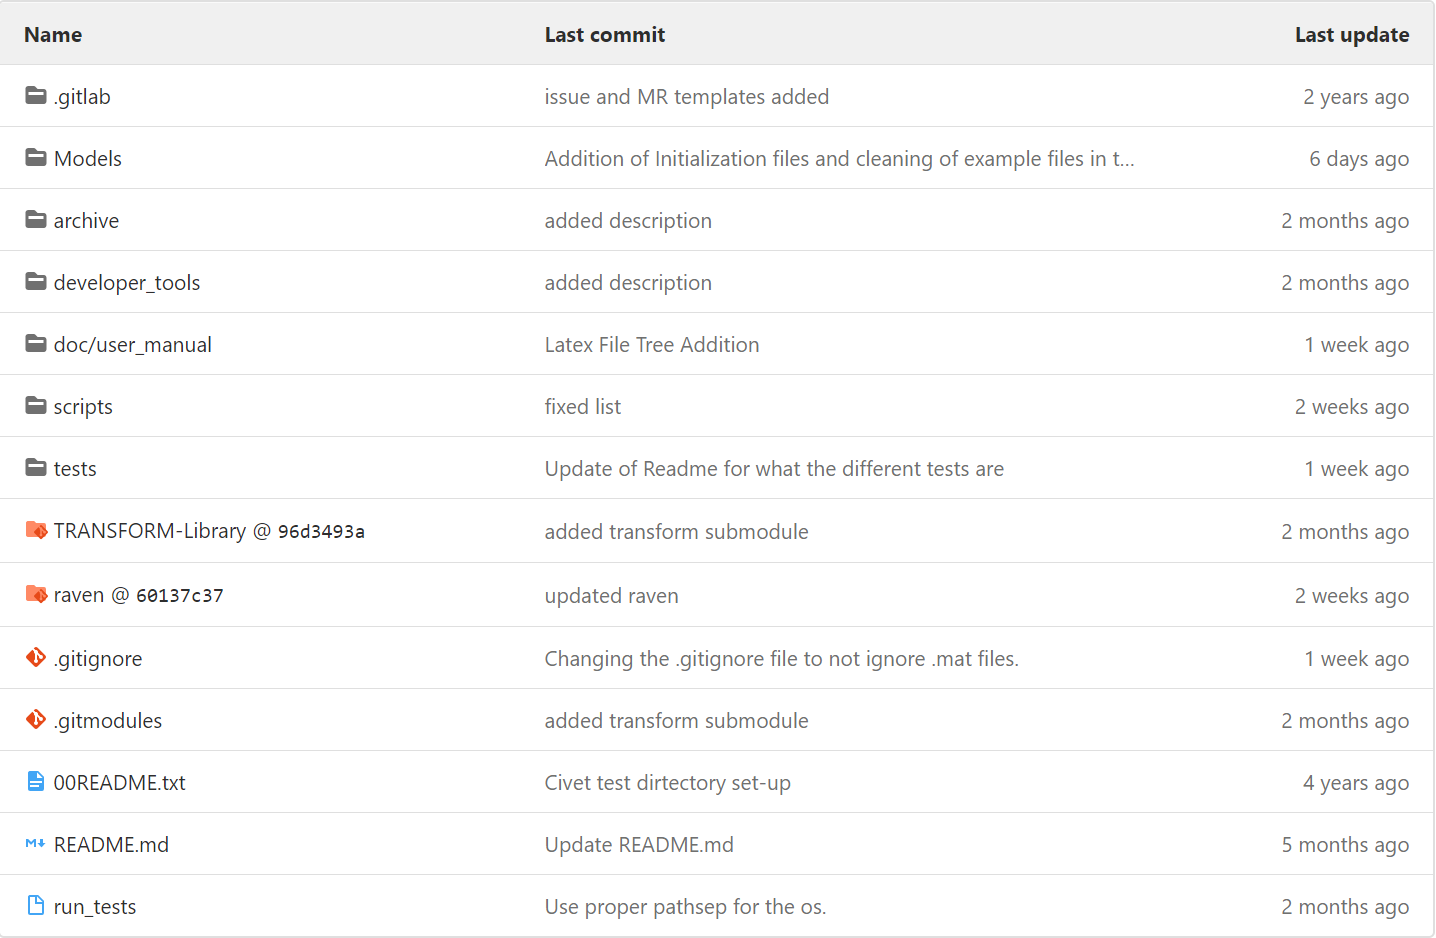
\includegraphics[scale=0.4]{pics/Repository_Structure.png}
\caption{Structure of the HYBRID repository.}
\end{figure}

\subsection{Regression Test System}
HYBRID a repository that contains a series of Modelica models capable of producing potential integrated energy system configurations. To test these models the RAVEN based regression system ROOK has been utilized. This testing system has been linked with the Continuous Integration tool to automatically test the models when new modifications are added to the repository. To do this RAVEN has been sub-moduled within HYBRID. 

\subsubsection{Dymola Regression Tests}
ROOK operates via a basic testing harness. The testing harness includes a “tests” file that contains the tolerance limits, a gold folder with a gold test file, a simulation file to run, a file with which to launch the simulation, and a directory of tests to run. Since the models to be run are Modelica models within the Dymola simulation platform a dymola\textunderscore launcher file was created to automatically run Dymola via the command line interface. For Modelica models the gold file is checked via a .mat file differ that has been created within the ROOK testing harness. This .mat differ checks all variables created by the test and compares them with an earlier version of the system. If the new .mat file is within a specified “tolerance” then the testing harness comes back with a clean pass.  A series of Modelica tests have been added to test the system-level interactions in the Nuclear Hybrid Energy Systems (NHES) Modelica repository and the collection of regression tests will continue to grow as the number of models and model uses grows.

\subsubsection{Raven "Hybrid Specific" Regression Tests}
In addition to the Modelica testing conducted by ROOK additional RAVEN specific tests are run. These raven tests are of workflows that are specific to hybrid energy system workflow generation. HYBRID is designed to be able to provide a techno-economic assessment of different integrated energy systems. As part of this HYBRID includes the generation of RAVEN workflows capable of implementing stochastic time series of wind, solar, and electric price data created via the Auto Regressive Moving Averages (ARMAs) algorithms within RAVEN into a workflow that can then be integrated into the Modelica models. The creation of these ARMAs using data held within the HYBRID repository is maintained using the ROOK system. 



\section{Data Design and Control}
The data transfer in the HYBRID framework is fully standardized:
\begin{itemize}
  \item  \textbf{\textit{Modelica Models}}: API deployed by Modelica Models;
  \item \textbf{\textit{FMI/FMU}}: API deployed by the FMI/FMU importer/exporter for RAVEN and Modelica models.
\end{itemize}
The documentation of these APIs is reported in the HYBRID user manual.

\section{Human-Machine Interface Design} 
 There are no human system integration requirements associated with this software.
 \section{System Interface Design} 
HYBRID framework contains Modelica models that can be interfaced directly by modelica packages (e.g. Dymola) or
via the standardized FMI/FMU interface.

 \section{Security Structure} 
The software is accessible to the open-source community (Apache License, Version 2.0). No restrictions for downloading or redistributing is applicable.

 \section{REQUIREMENTS CROSS-REFERENCE} 
The requirements are detailed in SPC-2990, ``HYBRID Software Requirements Specification (SRS) and Traceability Matrix''.




    % ---------------------------------------------------------------------- %
    % References
    %

\addcontentsline{toc}{section}{References}
\bibliographystyle{ieeetr}
\bibliography{software_design_description}

\section*{Document Version Information}

cb7e68b7e1757a4b957e18af7a6bdaa613d514b3 klfrick2 Mon, 15 Feb 2021 09:01:17 -0700


\end{document}
